\red{\begin{itemize}
\item more about software?
\item information pertaining to future test flights

\end{itemize}}


\subsection{Why Transition?}
In order to complete the objectives, long range flight would be required. This is why a transition system was necessary to implement, allowing the VTOL drone to fly forwards, both faster and more efficiently. This will hopefully allow the drone to fly for the required 1 hour flight time needed in deliverable 2, and allow it to travel for over 60 km that is required for the task. 

\subsection{Forward flight}
The plane was designed from the beginning to deal with transition. It was decided that two propellers of the VTOL copter would rotate forwards, creating a forward thrust and generating lift on the wings.  
\\\\
Firstly, a combination of wings and front motors capable of forward flight were required.  As mentioned the Skywalker X8 was shown to work well with forward flight, and the motors chosen (Turnigy SK3-3542-800) were the same chosen by others online, some who have achieved over 142km of flight time with the Skywalker(link?). eCalc (see Appendix \ref{sec:ecalc}, Figure \ref{fig:fixed}) suggested that at 3.5kg the aircraft had an estimated stall speed of 32km/h and a cruising speed of 82km/h with this combination. Additional calculations (see \ref{sec:stall}) further verified flight by ensuring a worst case stall speed at 4kg, with the Skywalker's minimum coefficient of lift for level flight at 0.5, of 45.5km/h. As the air will be forced over the wing, it is believed this should create further lift.

\subsection{Gyroscopic Forces}
An analysis of the gyroscopic forces acting on the motors during transition was performed to determine the required configuration of the motors, the strength of the shaft in between the two motors, and the torque required to make the transition. The calculations (see Appendix  \ref{sec:gyro}) showed that gyroscopic forces would create a moment perpendicular to the direction of rotation based on the direction of the motor angular velocity. To counteract this, two propellers on the front spinning in opposite directions would create zero net moment, and therefore the drone would be able to remain steady after transition. This was already the plan as counter rotating propellers also create a zero net angular momentum from the front in VTOL mode, making control much easier.\\

From this, the total moment created by this gyroscopic motion was 3.1Nm in the centre of the shaft, however for our rotation speed, this was less than the moment gravity exerted on the shaft while the motors were hovering, which was 9.156Nm. Lastly, the transition system would need to hold the propellers steady for any other gyroscopic forces. In particular if the aircraft rolls too fast, it would create a moment in the front. Due to the counter-rotating front motors however, these forces again would be opposite and counteracting.\\

The front servo would therefore receive no counter moment in flight. An arbitrary servo was chosen at 8.65kg/cm (0.85Nm), through testing it was found to behave satisfactorily against frictional or other unknown forces. This was verified by holding the drone down in tests and ensuring transition was possible at full motor speed.

\subsection{System Design}
For implementation a 1:1 gear \red{ref to gears section in appendix} system attached between the servo and motor shafts was installed (see Figure \ref{fig:gearsys}). This allowed for full rotation of the servo, and maximum accuracy.  Through testing of PWM values, it was set up to rotate by 90 degrees as required. A new mode was created through the open source Pixhawk firmware called “Fixed-Wing”, and possible transition from the VTOL modes was also set-up. This was created such that when a switch on the controller is turned, the front pole and motors rotate forwards 90 degrees, the VTOL control systems turn off, and the fixed wing control systems take over.\\

\begin{figure}[!ht]
	\centering
	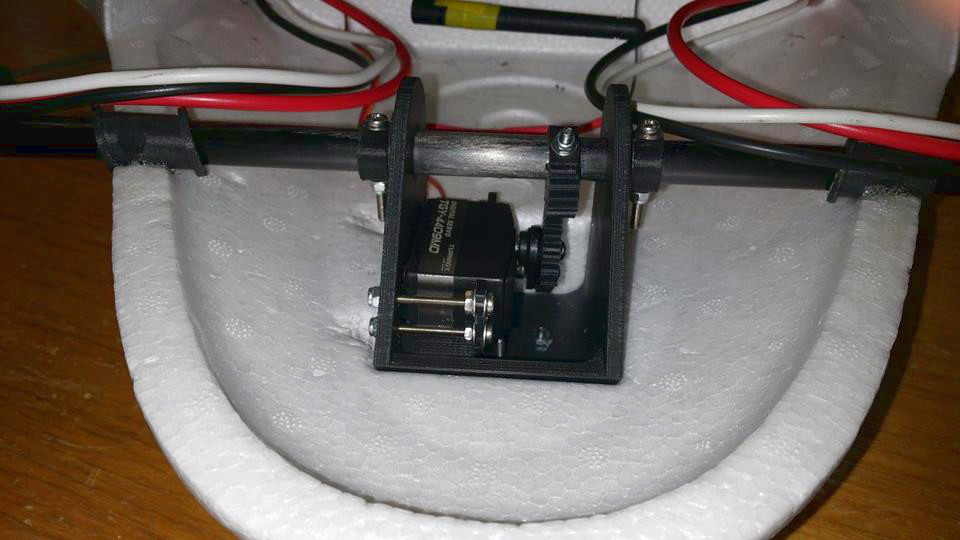
\includegraphics[width=300pt]{\IMAGEPATH /Prototype/gear_system}
	\caption{Front gear and mounting system}
	\label{fig:gearsys}
\end{figure}

So far, a manual fixed wing mode has been created. It turns off VTOL control systems and changes the user input from controlling the rotation of the multi-copter, to the control surfaces of the aircraft when entering this mode. This meant programming such that pulling down or up on the left stick meant the flaps move up and down respectively for pitch, and moving the right stick moves the flaps in opposite direction for roll.  In order to implement this changes to the firmware were required.  This meant having  a complete understanding of the programming behind both the Pixhawk \red{ref to PixHawk dev} and the open source ArduPilot project \red{ref ArduPilot dev}, and it also meant contributions were made to this open source platform. Eventually other modes would need to be created to complete the task, such as automated modes, or modes with basic stability control.\\

\subsection{Testing}
A number of steps needed to be taken to transition into fixed wing mode: 
\red{given manual transition controls}
\todomessage{firefly instruction vid reference https://www.youtube.com/watch?v=VPUSLzj02dA}

\begin{itemize}
\item In altitude hold keep the throttle at 50\% and move the aircraft forwards to create some initial speed
\item At a stable but fast speed level the aircraft
\item Flick the transition switch 
\item Lower the throttle
\item Pull up and raise the throttle as required

Once the system were built, off-line tests were conducted by holding the aircraft down and rotating the front rotors while at hover speed. Control surfaces on the wings were also tested. 

\todomessage{actual transition results}
		
\end{itemize}
